\documentclass[a4paper, 10pt, oneside, DIV=9, chapterprefix=true, numbers=enddot,bibliography=totoc]{scrbook}

\RedeclareSectionCommand[tocdynnumwidth]{chapter}
\RedeclareSectionCommands[tocdynindent]{section,subsection}
\usepackage{styleAT1}
\usepackage{shortcutsAT1}
\usepackage[normalem]{ulem}
\usepackage[outline]{contour}
\contourlength{2.25pt}

\newcommand{\embrace}[1]{\textup{(}#1\textup{)}}
\newlength{\LETTERheight}
\AtBeginDocument{\settoheight{\LETTERheight}{I}}
\newcommand*{\longrightsquigarrow}[1]{\ \raisebox{0.24\LETTERheight}{\tikz \draw [-to,
		line join=round, line cap=round,
		decorate, decoration={
			zigzag,
			segment length=4,
			amplitude=.9,
			post=lineto,
			post length=0.42ex
		}] (0,0) -- (#1,0);}\ }
	
\newlength{\HeightOfTextstyleOne}
\settoheight{\HeightOfTextstyleOne}{$\mathbf{1}$}
\newlength{\HeightOfScriptstyleOne}
\settoheight{\HeightOfScriptstyleOne}{$\scriptstyle\mathbf{1}$}
\newlength{\HeightOfScriptscriptstyleOne}
\settoheight{\HeightOfScriptscriptstyleOne}{$\scriptscriptstyle\mathbf{1}$}
\newcommand{\FancyOne}[1]{{\tikz[line cap=round,line join=round,line width=0.35*#1/\HeightOfTextstyleOne,scale=#1/\HeightOfTextstyleOne]{\draw (-0.0225,0.205) to (-0.0225,0.02) to[out=270,in=0] (-0.0425,0) to (-0.071,0) to (0.071,0) to (0.0425,0) to[out=180,in=270] (0.0225,0.02) to (0.0225,0.235) to (0.0175,0.235) to[out=210,in=0] (-0.075,0.201);}}}
\newcommand{\IOne}{\mathchoice%
	{\FancyOne{\HeightOfTextstyleOne}}%
	{\FancyOne{\HeightOfTextstyleOne}}%
	{\FancyOne{\HeightOfScriptstyleOne}}%
	{\FancyOne{\HeightOfScriptscriptstyleOne}}%
}
\newcommand{\IDigamma}{\tikz[line cap=round,line join=round,line width=0.35]{\draw (0.06,0.2286) to[out=0,in=90] (0.1353,0.172) to (0.1353,0.2286) to (-0.0525,0.2286) to (-0.0415,0.2286) to[out=0,in=90] (-0.0215,0.2086) to (-0.0215,0.02) to[out=270,in=0] (-0.0415,0) to (-0.0525,0) to (0.0605,0) to (0.0415,0) to[out=180,in=270] (0.0215,0.02) to (0.0215,0.2086) to[out=90,in=180] (0.0415,0.2286);\draw (0.025,0.1335) to[out=0,in=90] (0.0968,0.0769) to (0.0968,0.1335) to cycle;}\hspace{0.1ex}\vphantom{\IF}}

\newcommand{\sk}{\operatorname{sk}}
\newcommand\Yo{Y}%{\text{\usefont{U}{min}{m}{n}\symbol{'210}}\hspace{-0.125ex}\vphantom{Y}}
\newcommand{\add}{\mathrm{add}}
\newcommand{\Catst}{\Cat_\infty^\mathrm{st}}
\newcommand{\Verd}{\mathrm{Verd}}
\newcommand{\Kar}{\mathrm{Kar}}

\DeclareFontFamily{U}{min}{}
\DeclareFontShape{U}{min}{m}{n}{<-> udmj30}{}

	
\makeatletter
\renewcommand{\@pnumwidth}{2em} 
\renewcommand{\@tocrmarg}{3em}
\makeatother
%\RedeclareSectionCommand[tocindent+=0.5em]{section}
%\RedeclareSectionCommand[tocindent+=0.5em]{subsection}


\subject{Lecture Notes for}
\title{Algebraic Topology I}
\author{{\normalsize Lecturer}\\
	Stefan Schwede}
\date{{\normalsize Notes typed by}\\
	Michele Lorenzi}
\publishers{Winter Term 2021/22\\
	University of Bonn}

\usepackage{bookmark}
\begin{document}

\setlength{\parindent}{0pt}
\setlength{\parskip}{4pt}

\frontmatter
\KOMAoption{chapterprefix}{false}
\renewcommand{\thedummy}{\arabic{dummy}}
\maketitle
This document will (hopefully) contain lecture notes for the course \emph{Algebraic Topology I} given by Prof. Stefan Schwede at Bonn University during the winter semester 2021/22.

Thanks to \'Alvaro for the illustrations!

Everything in these notes should be taken with a grain of salt (at least for now), I'm new to the material, to real time \TeX ing and I tend to be late to class more often than not.

Eventually I plan to make these notes into a nice reference, maybe adding some (well written) solutions to some important exercises or useful comments, so if you have any correction/remark/suggestion on how to improve the notes, that would be much appreciated.

Also a lot of thanks to Paul, Yikai, Zhu, for lending me their notes/photos of the blackboard when I was missing stuff.

\hrulefill

Last update: \today
	
%Some additions have been made by the author. To distinguish them from the lecture's actual contents, they are labelled with an asterisk. So any \emph{Proof}* or \emph{Lemma}* etc.\ that the reader might encounter are wholly the author's responsibility.
%\\[\thmsep]Please report errors, typos etc.\ through the \href{https://github.com/}{\emph{Issues}} feature of GitHub, or just tell me before or after the lecture.
	
	
\tableofcontents
\listoftoc{lol}
\setcounter{llecture}{0}
\mainmatter\KOMAoption{chapterprefix}{true}
\renewcommand{\thedummy}{\thechapter.\arabic{dummy}}
\renewcommand{\thechapter}{\arabic{chapter}}
%%% Lecture 1

\renewcommand{\thechapter}{\Roman{chapter}}

\chapter{Hurewicz Theorem}

\section{Introduction}

\lecture[Introduction and first encounter with Hurewicz theorem.]{2021-10-11}

In the Topology I class given by Prof. Schwede last year, two important homotopy invariant functors were defined:

\begin{itemize}
    \item The singular homology groups $H_n(X;\Z)$. The definition of these groups is quite involved, but they are relatively easy to compute (e.g. by cellular homology). In the case of the spheres we have:
    \[\til{H}_n(S^k;\Z)=\begin{cases*}\Z & if $n=k$ \\ 0 & otherwise\end{cases*}\]
    
    \item The homotopy groups $\pi_n(S^k,*)$. These groups are instead easy to define, but really difficult to compute. In the case of the spheres their calculation becomes complicated already for $n>k$:
    \[\pi_n(S^k)=\begin{cases*}0 & if $n<k$ \\ \Z & if $n=k$ \\ ??? & if $n>k$\end{cases*}\]
    
    As of today (and most likely as of tomorrow too) still a lot is unknown about the higher homotopy groups of the spheres, and those we do know display an apparently erratic behaviour.
\end{itemize}

Homotopy groups are so hard to compute in general that, as a matter of fact, \emph{there is no non-contractible, simply connected finite CW-complex for which all homotopy groups are known.}

\section{A First Look to Hurewicz Theorem}

An important result about homotopy groups is a theorem due to Hurewicz relating the first non-trivial homotopy and homology groups under certain hypotheses:

\begin{theorem}[Hurewicz]\label{theorem:absolute-hurewicz}
Let $n\geq2$ and let $X$ be an $(n-1)$-connected based space. Then $H_i(X;A)=0$ for all $0<i<n$ and any abelian group $A$ and the Hurewicz map
\[h:\pi_n(X,x_0)\to H_n(X;\Z)\]
is an isomorphism.
\end{theorem}

Where the \textbf{Hurewicz map} is defined in the following way. Let $n\geq1$ and let $c\in H_n(S^n;\Z)$ be a generator. For a based space $(X,x_0)$ define
\[h:\pi_n(X,x_0)\to H_n(X;\Z),\ [f:S^n\to X]\mapsto f_*(c)\]
where $f_*:H_n(S^n;\Z)\to H_n(X,\Z)$ is the map induced by $f$ on homology groups. I.e. the Hurewicz map $h$ is the evaluation at the fundamental class of $S^n$.

Proving this theorem will keep us busy for the next few lectures.

\begin{remark}
Choosing the other generator of $H^n(S^n;\Z)$, the Hurewicz map changes into its negative which is still an isomorphism, i.e. the map itself slightly depends on the choice of the generator, but the fact that it is an isomorphism does not.
\end{remark}

\begin{remark}
Recall: for path connected $X$, $h:\pi_1(X,x_0)\to H_1(X,\Z)$ is surjective with kernel the commutator subgroup, so it factors to an isomorphism $\pi_1(X,x_0)^{\text{ab}}\to H_1(X;\Z)$. The Hurewicz theorem is a generalization of this fact, whose first proof is due to Poincaré.
\end{remark}

We know prove two properties of the Hurewicz map, namely its naturality and the fact that it is actually a group homomorphism.

\unnumpar{Naturality of the Hurewicz map} Let $f:X\to Y$ be a based map between based spaces. Then the following square commutes
\begin{center}
    \begin{tikzcd}
        \pi_n(X,x_0) \arrow[r, "h^X"] \arrow[d, "f_*"] & H_n(X;\Z) \arrow[d, "f_*"] \\
        \pi_n(Y,f(x_0)) \arrow[r, "h^Y"] & \pi_n(Y;\Z)
    \end{tikzcd}
\end{center}

\begin{proof}
Let $\alpha:S^n\to X$ represent a class in $\pi_n(X,x_0)$. Then
\[f_*(h^X[\alpha])=f_*(\alpha_*(c))=(f\alpha)_*(c)=h^Y[f\circ\alpha]=h^Y(f_*[\alpha])\]
\end{proof}

\unnumpar{The Hurewicz map is a group homomorphism} Let $p:S^n\to S^n\vee S^n$ be a pinch map\marginnote{\footnotesize The pinch map is the subject of one of the exercises in the first exercise sheet ("The" pinch map, because as we will see it is unique up to homotopy).}, i.e. a continuous based map such that both compositions with the projections $S^n\vee S^n\rightrightarrows S^n$ are based-homotopic to the identity. The group structure on $\pi_n(X,x_0)$ (for $n\geq2$) is as follows (thinking of spheres):
\[[f]+[f']:=[(f\vee f')\circ p].\]
It will be an exercise this week to show that if $i_1,i_2:S^n\to S^n\vee S^n$ are the two summand inclusions the following relations holds:
\[p_*(c)=(i_1)_*(c)+(i_2)_*(c) \text{ in } H_n(S^n\vee S^n;\Z)\]
with $c\in H_n(S^n;\Z)$ generator.
Now we can show that the Hurewicz map is in fact a group homomorphism.
\begin{proof}
If $[f],[f']\in\pi_n(X,x_0)$ we have:
\[h([f]+[f'])=h[(f\vee f')\circ p]=((f\vee f')\circ p)_*(c)=(f\vee f')_*(p_*(c))=(f\vee f')_*((i_1)_*(c)+(i_2)_*(c)_*)\]
but since $(f\vee f')\circ i_1=f$ and $(f\vee f')\circ i_2=f'$,
\[(f\vee f')_*((i_1)_*(c))+(f\vee f')_*((i_2)_*(c)_*)=f_*(c)+f'_*(c)=h[f]+h[f']\]
\end{proof}

We will actually prove a stronger version of the Hurewicz theorem, the relative Hurewicz theorem.

Recall the definition of the relative homotopy groups. We identify $I^\ni$ with the subspace of $I^n$ with $x_1=0$. Define $J^\ni=\de (I^n)\sm\mathring{I}^\ni$. Then $I^\ni\cap J^\ni=\de(I^\ni)$.
\begin{center}
    \(
    \begin{tikzcd}
    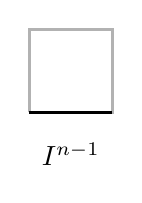
\begin{tikzpicture}[x=3em, y=3em, baseline=1em]
        \draw[very thick, black!30] (0,0)--(1,0)--(1,1)--(0,1)--(0,0);
        \draw[very thick]
        (0,0)--(1,0);
        \filldraw (0.5, -0.5) node{$I^{n-1}$};
    \end{tikzpicture}
    \ar[r, hook]
    &
    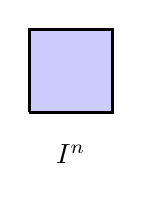
\begin{tikzpicture}[x=3em, y=3em, baseline=1em]
        \filldraw[very thick, fill=blue!20] (0,0)--(1,0)--(1,1)--(0,1)--(0,0);
        \filldraw (0.5, -0.5) node{$I^{n}$};
    \end{tikzpicture}
    & 
    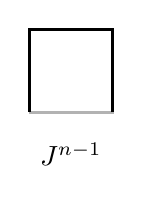
\begin{tikzpicture}[x=3em, y=3em, baseline=1em]
        \draw[very thick, black!30] (0,0)--(1,0)--(1,1)--(0,1)--(0,0);
        \draw[very thick] (1,0)--(1,1)--(0,1)--(0,0);   \filldraw (0.5, -0.5) node{$J^{n-1}$};
    \end{tikzpicture}
    \ar[l, hook]
    \end{tikzcd}
    \)
\end{center}
The \textbf{relative homotopy groups} of the triple $(X,A,x_0)$ are defined as triple homotopy classes of triple maps:
\[\pi_n(X,A,x_0)=[(I^n, I^\ni, J^\ni),(X,A,x_0)].\]
Addition on $\pinr$ for $n\geq 2$ is defined by "juxtaposition and reparametrization in the first coordinate" as follows:
\[[f]+[g]=[f+g],\ (f+g)(\nn{t}{n})=\begin{cases}f(2t_1,\dots,t_n) & t_1\in[0,1/2] \\ g(2t_1-1,\dots,t_n) & t_1\in[1/2,1]\end{cases}\]
this is easily seen to be well defined on homotopy classes.

The \textbf{relative Hurewicz map} is defined similarly to the absolute one: with $c\in H_n(I^n,\de I^n;\Z)$ a generator, define
\[h:\pi_n(X,A,x_0)\to H_n(X,A;\Z),\ [f]\mapsto f_*(c)\]


Recall that $\pi_1(A,x_0)=[(I',\de I'),(A,x_0)]$ acts on $\pi_n(X,A,x_0)$ in a non-trivial fashion. This poses a problem, because for all $[f]\in\pi_n(X,A,x_0)$ and $\omega\in\pi_1(S,x_0)$ the maps representing $[\omega]*[f]$ and $[f]$ are pair-homotopic as maps $(I^n,\de I^n)\to(X,A)$, hence the relative Hurewicz map takes them to the same class in $H_n(X,A;\Z)$.

This leads to the definition of a \textbf{modified relative Hurewicz map}. For $n\geq2$ define $\pinr^\dagger$ to be the quotient of $\pinr$ by the normal subgroup generated by elements of the form $([\omega]*[f])[f]^{-1}$ for all $[\omega]\in\pi_1(A,x_0)$, $[f]\in\pinr$. By design the relative Hurewicz map factors through this quotient:
\begin{center}
    \begin{tikzcd}
        \pinr \arrow[r, "h"] \arrow[d] & \hnr \\
        \pinr^\dagger \arrow[ur, dashed, "h^\dagger" below]
    \end{tikzcd}
\end{center}

Now we can state the relative Hurewicz theorem.

\begin{theorem}[Hurewicz]\label{theorem:hurewicz}
Let $(X,A)$ be a pair of path connected spaces such that for all $x_0\in A$, the map $\pi_1(A,x_0)\to\pi_1(X,x_0)$ is an isomorphism. Let $n\geq2$ and suppose that $\pi_i(X,A,x_0)=0$ for $1\leq i\leq n-1$. Then the modified relative Hurewicz map $h^\dagger$ is an isomorphism.
\end{theorem}

\begin{remark}
For $A=\{x_0\}$, the relative version recovers the absolute version.
\end{remark}

\begin{remark}
The hypothesis of the relative Hurewicz theorem refers to $\pi_i(X,A,x_0)$ but the conclusion refers to $\pi_n(X,A,x_0)^\dagger$. This makes the relative version not as manageable as the absolute one.
\end{remark}
%%% Lecture 2

\section{Some Consequences of Hurewicz Theorem}

\lecture[Getting rid of the basepoint.]{2021-10-13}

Before resuming with the proof of the relative Hurewicz theorem we prove an application of it, a version of Whitehead's theorem which uses homology groups in place of homotopy groups.

\begin{theorem}
Let $f:X\to Y$ be a map between simply connected CW-complexes such that $f_*:H_i(X;\Z)\to H_i(Y;\Z)$ is an isomorphism for all $i\geq 0$. Then $f$ is an homotopy equivalence.
\end{theorem}

\begin{proof}
By cellular approximation we can assume $f$ cellular. Let $Z(f)=X\times[0,1]\cup_{X\times1, f}Y$ be the mapping cylinder of $f$. This inherits a CW-structure such that $X\cong X\times0$ and $Y$ are subcomplexes. The projection $Z(f)\to Y$ is a homotopy equivalence (fact check this), hence by replacing $Y$ by $Z(f)$ we can assume wlog that $f:X\to Y$ is the inclusion of a subcomplex. Since $X$ and $Y$ are simply-connected the relative Hurewicz theorem applies for all $n\geq2$, but all relative homology groups vanish because $f_*$ is an isomorphism (by the long exact sequence), hence all relative homotopy groups vanish and by Whitehead's theorem we can conclude that $f$ is an homotopy equivalence.
\end{proof}

An elaboration of the previous results leads to the following proposition.

\begin{proposition}
Let $f:X\to Y$ be a map of path-connected CW-complexes. The following are equivalent:
\begin{itemize}
    \item[(i)] $f$ is a homotopy equivalence,
    \item[(ii)] $f$ induces an isomorphism on fundamental groups and the induced map $\til{f}:\til{X}\to\til{Y}$ on universal covers induces an isomorphism on all integral homology groups.
\end{itemize}
\end{proposition}

\begin{proof}
$(i)\implies(ii)$ Since $f$ is an homotopy equivalence, $f_*$ is an isomorphism on all homotopy groups. Then $\til{f}$ induces an isomorphism on all homotopy groups, hence it is an homotopy equivalence, thus it induces an isomorphism on all homology groups.

$(ii)\implies(i)$ Since $\til{f}$ induces an isomorphism on integral homology groups it is a homotopy equivalence by the version of Whitehead's theorem we just proved, hence it induces an isomorphism on all homotopy groups. This in turn means that $f$ induces an isomorphism on all homotopy groups, i.e. it is a homotopy equivalence.
\end{proof}

\section{Getting Rid of the Basepoint}

We now return to the proof of the relative Hurewicz theorem

Recall: the \textbf{degree} of a map $f:(D^n,\de D^n)\to(D^n,\de D^n)$ is the integer $\deg(f)$ such that $f_*(x)=\deg(f)x$ for all $x\in H_n(D^n,\de D^n;\Z)$.

\begin{lemma}\label{lemma:degree-of-sphere-self-maps}
Let $n\geq1$. For $n>1$ assume known that $\pi_\ni(\sni,z)$ is free abelian of rank $1$. Let $f$ be a continuous self map of $\sph$ of degree $\pm 1$. Then $f$ is pair-homotopic to the identity if $\deg(f)=1$ and to any reflection if $\deg(f)=-1$.
\end{lemma}

\begin{proof}
We first see the case when $\deg(f)=1$.

$(n=1)$ Since $\de D^1=\cb{\pm1}$ and $\deg(f)=1$ we have $f|_{\de D^1}=\id_{\de D^1}$. Then the linear homotopy $H(x,t)=tf(x)+(1-t)x$ is a relative homotopy between $f$ and the identity $id_{D^1}$.

$(n\geq2)$ Consider the commutative square:
\begin{center}
    \begin{tikzcd}
    H_n(\dn,\de\dn;\Z) \arrow[d,"f_*=\id"] \arrow[r, "\de", "\cong" below] & H_\ni(\sni;\Z) \arrow[d, "(f|_{S^\ni})_*=\id"] \\
    H_n(\dn,\de\dn;\Z) \arrow[r, "\de", "\cong" below] & H_\ni(S^\ni;\Z)
    \end{tikzcd}
\end{center}
Since $\pi_\ni(S^\ni,z)$ is free of rank $1$, the Hurewicz map $h:\pi_\ni(S^\ni,z)\to H_\ni(S^\ni;\Z)$ is an isomorphism. Then $(f|_{\de\dn})_*:\pi_\ni(\sni,z)\to\pi_\ni(\sni,z)$ is the identity, therefore $f|_{\de\dn}$ is homotopic to the identity of $\sni$. Now let $H:\sni\times [0,1]\to\sni$ be a homotopy. This gives a map $D^n\times0\cup\sni\times[0,1]\cup \dn\times1\xto{f\cup H\cup\id}\dn$. Since $\dn\times[0,1]$ can be obtained from $D^n\times0\cup\sni\times[0,1]\cup \dn\times1$ by attaching an $(n+1)$-cell and $\dn$ is contractible\normalmarginpar\marginnote{\footnotesize Why do we need $\dn$ contractible? Think of $S^1\hookrightarrow D^2$}, there is a continuous extension $\bar{H}:\dn\times[0,1]\to\dn$. This is the desired pair homotopy from $f$ to $\id_{\dn}$.

If $\deg(f)=-1$, we let $r:\dn\to\dn$ be the reflection in the first coordinate. Then $\deg(r\circ f)=1$, hence $r\circ f$ is pair homotopic to $\id_{\dn}$ and so $f=r\circ r\circ f$ is pair homotopic to $r$.
\end{proof}

Now let $(X,A)$ be a based space. Define the group $\pi_n(X,A)^\#$ as the quotient of the free abelian group generated by pair homotopic maps $(I^n,\de I^n)\to (X,A)$ by the relation $[f]+[f']=[f+f']$ when the right hand side is defined.

The "forgetful" map $\pinr\to\pi_n(X,A)^\#$ is a group homomorphism and it factors through a homomorphism $\pinr^\dagger\to\pi_n(X,A)^\#$ (because $\omega * f$ and $f$ are always pair homotopic).

\begin{proposition}
Let $(X,A)$ be a pair of path-connected spaces. Let $n\geq2$ or $n=1$ and $A$ a point. Then the "forgetful" homomorphism $\pinr^\dagger\to\pi_n(X,A)^\#$ is an isomorphism.
\end{proposition}

\begin{proof}
We will define a homomorphism in the opposite direction. Let $f:(I^n,\de I^n)\to (X,A)$ be a pair map. $f$ need not send $J^\ni$ to $x_0$, but $J^\ni$ is contractible and $A$ path-connected. So $f|_{J^\ni}$ is homotopic in A to the constant map at the basepoint. Let $H:J^\ni\times[0,1]\to A$ be such a homotopy from $f|_{J^\ni}$ to the constant map $x_0$. The HEP for $(\de I^n,J^\ni)$ lets us extend $H$ to a homotopy $H':\de I^n\times[0,1]\to A$ from $f|_{\de I^n}$ to some map $H'(1,-)$ that sends $J^\ni$ to $x_0$. The HEP for $(I^n,\de I^n)$ with target space $X$ lets us extend $H'$ to $H'':I^n\times[0,1]\to X$ from $f$ to a map that sends $J^\ni$ to $x_0$. Moreover $H''$ is a pair homotopy of maps $(I^n,\de I^n)\to (X,A)$.

We now define a map $\Psi:[(I^n,\de I^n)\to (X,A)]\to \pi_n(X,A,x_0)^\dagger$ by sending $[f]$ to $[H''(-,1)]$. We claim that this is well defined.
 
Claim. Let $f,f':(I^n,\de I^n, J^\ni)\to(X,A,x_0)$ be triple maps that are pair homotopic as maps $(I^n,\de I^n)\to (X,A)$. Then they represent the same element in $\pi_n(X,A,x_0)^\dagger$.
 
\textit{Proof of the claim.} Let $H:I^n\times[0,1]\to X$ be a pair homotopy from $f$ to $f'$. We choose a point $z\in J^\ni$ and a triple homotopy $K:\triple\times[0,1]\to\triple$ from the identity to a map with $K(J^\ni\times 1)=\{z\}$. Formally what we are applying two times the HEP (for $(\de I^n,J^\ni)$ and for $(I^n,\de I^n)$, as before). Then $f$ is triple homotopic to $f\circ K(-,1)$, $f'$ is triple homotopic to $f'\circ K(-,1)$, so that $f\circ K(-,1)$ is pair homotopic to $f'\circ K(-,1)$. In particular $\til{H}=H \circ K(-,1)$ satisfies $\til{H}(J^\ni,t)=H(z,t)$ for all $t\in [0,1]$. Now for all $x\in J^\ni$, the loop at $x_0$ in $A$, $\til{H}(x,-)$, is independent of the point $x\in J^\ni$ and it always agrees with $\omega=\til{H}(z,-)$. By identifying $I^{n+1}$ as $I^n\times[0,1]$ we can view $\til{H}$ as a triple homotopy between $\omega * (f\circ K(-,1))$ and $f'\circ K(-,1)$.\normalmarginpar\todo{I'm not \textit{too} sure I really get this...} In the end we have $[f]=[\omega * (f\circ K(-,1))]=[f'\circ K(-,1)]=[f']$ in $\pinr^\dagger$ (the second equality holds in $\pinr^\dagger$ by construction, the third one is because of the homotopy we found).

\textit{Corollary of the claim.} The map $\Psi:[(I^n,\de I^n),(X,A)]\to\pinr^\dagger$ we defined before the claim is well defined, so it has a unique extension on the free abelian group which factors to a homomorphism $\pi_n(X,A)^\#\to\pinr^\dagger$ which is then an isomorphism by design.
\end{proof}
 
Punchline: In the situation of the relative Hurewicz theorem it suffices to show that the map $\pi_n(X,A)^\#\to H_n(X,A;\Z)$ is an isomorphism (i.e. we don't have to deal with basepoints!).

%%% Lecture 3

\section{The Homotopy Addition Theorem}

\lecture[The Homotopy Addition Theorem: a theorem which is necessary, but a pain to prove.\newline---\emph{\enquote{When homotopy theory was new, people thought this was obvious and didn't feel the need for a proof, until Eilenberg suggested so.}}]{2021-10-18}

This lecture was given by Tobias Lenz, a PhD student of Schwede. I was late to the class, so most of the notes for this lecture are copied from Qi Zhu's notes, thank you Qi Zhu!

\begin{remark}
There's a standing assumption for all of today's lecture: $\pi_k(S^k)\cong\Z$ for all $1\leq k<n$.
\end{remark}

The main goal of today's lesson is to prove the following theorem.

\begin{theorem}[Homotopy Addition Theorem]\label{theorem:HAT}
Assume we have $\nn{f}{k}:I^n\to I^n$ such that $f_i|_{\ring I^n}$ is an open embedding and the sets $f_i(\ring I^n)$ are pairwise disjoint. Furthermore, let $g:\pair\to (X,A)$ such that $g(I^n\sm\bigcup_{i=1}^k f_i(\ring I^n))\subset A$. Then
\[[g]=\sum_{i=1}^k(\deg f_i)[g\circ f_i]\]
in $\pi_n(X,A)\#$.
\end{theorem}

\begin{remark}
Note that we have $f_i(\de I^n)\cap f_j(\ring I^n)=\emptyset$ for all $i,j$. This will play a (small) role later in the lecture.
\end{remark}

\begin{remark}
Two remarks about the theorem:
\begin{itemize}
    \item When homotopy theory was new, people thought this was obvious and didn't feel the need for a proof until Eilenberg suggested so.
    \item Tobias: \emph{\enquote{I'm not sure if I can finish the proof today but I was promised an award if I do!}}
\end{itemize}
\end{remark}

\begin{center}
\begin{tikzpicture}[x=1.5em, y=1.5em]
\filldraw[very thick, black, fill=blue!20]
    (0,0)--(0,10)--(10,10)--(10,0)--(0,0);
\draw[very thick]
    (-4,4)--(-4,6)--(-2,6)--(-2,4)--(-4,4)
    (-4,1)--(-4,3)--(-2,3)--(-2,1)--(-4,1)
    (-4,7)--(-4,9)--(-2,9)--(-2,7)--(-4,7);
\filldraw[fill=white, use Hobby shortcut,closed=true] 
    (1,5) .. (4,9) .. (7,5) .. (4,8) .. (3,4) .. (5,2) .. (7,5) .. (8,2) .. (5,1);
\filldraw[fill=white, use Hobby shortcut,closed=true] 
    (3,5) .. (3,6) .. (5.3,6) .. (5.4,4);
\path[draw]
    (3,5) -- (3.5,5) -- (3.6,5.5) -- (3.8, 5.5);
\filldraw[fill=white, use Hobby shortcut,closed=true] 
    (8,1) .. (8,2) .. (9.5,2) .. (9.5,1);
\path[draw, -{\tip}, use Hobby shortcut,closed=false]
    (9,7) .. (9.5,7.5) .. (11,8);
\draw 
    (7,6) node {\scriptsize$f_1(I^n)$}
    (8.7,1.5) node {\scriptsize$f_2(I^n)$}
    (4.7,4.9) node {\scriptsize$f_3(I^n)$}
    (11,8) node[anchor=west] {$A$}
    (10,5) node[anchor=west] {$\xrightarrow{\quad g\quad} X$}
    (-2,2) node[anchor=west] {$\xrightarrow{\ f_1\ }$}
    (-2,5) node[anchor=west] {$\xrightarrow{\ f_2\ }$}
    (-2,8) node[anchor=west] {$\xrightarrow{\ f_3\ }$};
\end{tikzpicture}
\end{center}\label{fig:HAT1}\medskip

The strategy to prove this theorem is inductive: we want to reduce the problem to the case $k=1$ which is easy.

\begin{definition}
Let $f:\ring I^n\to\ring I^n $ be an open embedding, $p\in\ring I^n$. We have that $f$ induces a commutative diagram:
\begin{center}
    \begin{tikzcd}
    H_n(\ring I^n,\ring I^n\sm\cb{p}) \arrow[r, "i_*"] \arrow[d, "f_*" left] \arrow[dr, "f_*"] & H_n(I^n,I^n\sm\cb{p}) & H_n\pair \arrow[l, "i_*" above] \arrow[d, red, dashed, "d\cdot-"] \\
    H_n(f(\ring I^n), f(\ring I^n)\sm\cb{f(p)}) \arrow[r, "i_*" below] & H_n(f(I^n),f(I^n)\sm\cb{f(p)}) & H_n\pair \arrow[l, "i_*" below]
    \end{tikzcd}
\end{center}
\end{definition}
where the maps are all isomorphisms by homotopies and excision, hence they induce the dashed arrow. This is an automorphism of $H_n\pair\cong\Z$ and thus $d=\pm1$. One can show this is independent of $p$, hence we call it the \tbf{local degree} of $f$, and write $\deg(f)=d$.

\begin{lemma}
For $1\leq i\leq k$, let $\Uu_i\subset f_i(\ring I^n)$ be any non-empty open set. Then $g$ is homotopic relative to $I^n\sm f_i(\mathring{I}^n)$ to a map that sends $f_i(I^n)\sm\mathcal{U}_i$ to $A$ for all $i$.
\end{lemma}

\begin{remark}
If $[g]=[g']$ in $\pi_n(X,A)^\#$ then $[g\circ f_j]=[g'\circ f_j]$ for all $1\leq j\leq k$.
\end{remark}

\begin{proof}
There is a homotopy relative $\de I^n$ from the identity to a map that sends everything outside of $\ring Q$ to $\de I^n$, where $Q$ is a cube inside $f^{-1}_i(\mathcal{U}_i)$ (basically we take a cube $Q$ inside $f^{-1}_i(\mathcal{U}_i)$ and we blow it to the big cube $\de I^n$ containing $f^{-1}_i(\mathcal{U}_i)$). Composing with $gf_i$ yields a homotopy $H$ of maps of pairs $(I^n,\de I^n)\to(X,A)$ from $gf_i$ to a map that sends everything outside $\ring Q$ to $A$. We have a map of sets:
\[H':I^n\times I\to X,\quad H'(x,t)=\begin{cases}H(f^{-1}(x),t) & x\in f_i(I^n) \\ g(x) & x\not\in f_i(\mathring{I}^n)\end{cases}\]
which we can show is well defined. Let $x\in f_i(\de I^n)$, with preimage $y$, then\normalmarginpar\marginnote{\footnotesize It suffices to check this because $f_i(\de I^n)\cap f_j(\ring I^n)$ is empty for all $i,j$.} \[g(x)=H(y,t)=H(y,0)=gf_i(y)\] so that it is well defined as a map of sets. Then $H'(x,0)=g(x)$ and $H'(x,1)\in A$ for $x\not\in f(\mathring{Q})$, in particular $H'(x,1)\in A$ for $x\not\in\mathcal{U}_i$. It remains to prove that $H'$ is continuous.

Claim. We have a commutative square
\begin{center}
    \begin{tikzcd}[column sep=20mm]
    \de I^n\times I \arrow[d, "i"] \arrow[r, "f_i|_{\de I^n}\times\id"] & (I^n\sm f_i(\ring I^n))\times I \arrow[d, "i"] \\
    I^n\times I \arrow[r, "f_i\times\id"] & I^n\times I
    \end{tikzcd}
\end{center}
Then,
\[(I^n\times I)\amalg_{\de I^n\times I} ((I^n\sm f_i(\mathring{I}^n))\times I)\xto{(f_i\times\id,i)} I^n\times I\]
is a homeomorphism.

\begin{claimproof}
Well-definedness and continuity of the function follow from the universal property of the pushout. One can check that it is bijective by a direct computation. Hence we have a continuous bijection from a quasi-compact space to an Hausdorff space, which is then a homeomorphism. 
\end{claimproof}

Thus to show that $H'$ is continuous, it suffices to show that the maps $H'\circ (f_i\times I)$ and $H'|_{(I^n\sm f(\ring I^n))\times I}$ are continuous, which follows from the construction.\todo{Not sure how this works, to be honest}
\end{proof}

\begin{proof}[Proof of the homotopy addition theorem (\ref{theorem:HAT})]\renewcommand{\qedsymbol}{\textit{To be continued...}} Induction on $k$.

$(k=1)$ Take a cube $Z_1\subset f_1(\mathring{I}^n)$. By the lemma we may assume that $g(I^n\sm\mathring{Z}_1)\subset A$. Our goal is to construct some $f_1':(I^n,\de I^n)\to(I^n,\de I^n)$ with $[gf_1]=[gf_1']$. There exists\normalmarginpar\marginnote{\footnotesize The homotopy $Q$ is the same kind of "pushing out" homotopy that we already considered in the proof of the lemma.} a homotopy $Q$ from $\id_{I^n}$ to a map $p$ such that:
\begin{itemize}
    \item $p|_{Z}=\id_{Z}$, where $Z$ is a cube inside $Z_1$,
    \item $p(I^n\sm\mathring{Z}_1)\subset\de I^n$,
    \item $Q((I^n\sm\mathring{Z}_1)\times I)\subset I^n\sm \mathring{Z}_1$.
\end{itemize}
Now, $Qf_1$ is a homotopy of maps of pairs $(I^n,\de I^n)\to(I^n,I^n\sm\mathring{Z}_1)$. Then $gQf_1$ will be a homotopy of maps of pairs $(I^n,\de I^n)\to(X,A)$, hence $[gpf_1]=[gf_1]$ in $\pi_n(X,A)^\#$. Then $f_1':= pf_1$ is a map of pairs $(I^n,\de I^n)\to(I^n,\de I^n)$ and $f_1\simeq f_1'$ as maps of pairs $(I^n,\de I^n)\to(I^n,I^n\sm \mathring{Z}_1)$.

Claim.\reversemarginpar\marginnote{\footnotesize We are dealing with two different notions of degree, the usual one for $f'_1$ and the local degree for $f_1$.} $\deg f_1$ equals the degree of $f_1'$ as a map $(I^n,\de I^n)\to(I^n,\de I^n)$.

\begin{claimproof}
Consider the diagram:
\begin{center}
    \begin{tikzcd}[column sep=small]
    H_n(\mathring{I}^n,\mathring{I}^n\sm\cb{x}) \arrow[r, "i_*",] \arrow[d, "(f_1)_*" left] & H_n(I^n,I^n\sm\cb{x}) \arrow[d, "(f_1)_*"] & H_n(I^n,\de I^n) \arrow[l, "i_*" above] \arrow[d, shift left, "(f_1)_*\ \," left] \arrow[d, shift right, "\ \,(f'_1)_*" right] \arrow[dr, "(f'_1)_*"] \\
    H_n(\mathring{I}^n, \mathring{I}^n\sm\cb{f_1(x)}) \arrow[r, "i_*"] & H_n(I^n,I^n\sm\cb{f_1(x)}) & H_n(I^n,I^n\sm \mathring{Z}_1) \arrow[l, "i_*" above] & H_n\pair \arrow[l, "i_*"]
    \end{tikzcd}
\end{center}
we have that the parallel arrows agree, which proves the claim.
\end{claimproof}

Now, if $\deg f_1=1$, then $f_1'\simeq\id$ as maps of pairs, hence $(\deg f_1)[gf_1]=[gf_1']=[g]$.

If instead $\deg f_1=-1$, then $f_1'\sim r$ where $r$ is reflection in the first coordinate by lemma \ref{lemma:degree-of-sphere-self-maps}, hence $[g]=-[gr]=-[gf_1']=-[gf_1]=(\deg f_1)[gf_1]$.

\end{proof}

%%% Lecture 4

\lecture[We finish the proof of the HAT. My first non-trivial homotopy groups.]{2021-10-25}
$(k\geq2)$ Set $u_i=f_i(\text{center of } I^n)\in I^n$. Assume without loss of generality that the first coordinates of $\nn{u}{k}$ are not all equal (if some of them are, we can "wiggle" $f_1$).

\begin{center}
\begin{tikzpicture}[x=0.7em, y=0.7em, baseline=0.7*5em]
\filldraw[very thick, black, fill=blue!20]
    (0,0)--(0,10)--(10,10)--(10,0)--(0,0);
\filldraw[fill=white, use Hobby shortcut,closed=true] 
    (1,5) .. (4,9) .. (7,5) .. (4,8) .. (3,4) .. (5,2) .. (7,5) .. (8,2) .. (5,1);
\filldraw[fill=white, use Hobby shortcut,closed=true] 
    (4,5) .. (4,6) .. (5.3,6) .. (5.4,4);
\filldraw[fill=white, use Hobby shortcut,closed=true] 
    (8,1) .. (8,2) .. (9,2) .. (9,1);
\draw 
    (7,6) node {\scriptsize$f_1$}
    (8.5,1.5) node {\scriptsize$f_2$}
    (5.2,4.9) node {\scriptsize$f_3$};
\end{tikzpicture}
$\xrightarrow{\text{shrink domains to}}$
\begin{tikzpicture}[x=0.7em, y=0.7em, baseline=0.7*5em]
\filldraw[very thick, black, fill=blue!20]
    (0,0)--(0,10)--(10,10)--(10,0)--(0,0);
\filldraw[fill=white, use Hobby shortcut,closed=true] 
    (1,5) .. (2,6) .. (3,5) .. (2.5,3);
\filldraw[fill=white, use Hobby shortcut,closed=true] 
    (4,5) .. (4,6) .. (5.3,6) .. (5.4,4);
\filldraw[fill=white, use Hobby shortcut,closed=true] 
    (8,1) .. (8,2) .. (9,2) .. (9,1);
\draw[dashed] (3.5,0)--(3.5,10) (6.5,0)--(6.5,10);
\draw 
    (2,5) node {\scriptsize$f_1$}
    (8.5,1.5) node {\scriptsize$f_2$}
    (5.2,4.9) node {\scriptsize$f_3$};
\end{tikzpicture}
$\xrightarrow{\text{blow images to}}$
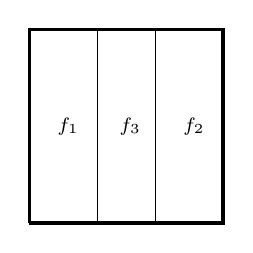
\begin{tikzpicture}[x=0.7em, y=0.7em, baseline=0.7*5em]
\draw[very thick, black]
    (0,0)--(0,10)--(10,10)--(10,0)--(0,0);
\draw (3.5,0)--(3.5,10) (6.5,0)--(6.5,10);
\draw 
    (2,5) node {\scriptsize$f_1$}
    (8.5,5) node {\scriptsize$f_2$}
    (5.2,5) node {\scriptsize$f_3$};
\end{tikzpicture}
\end{center}

\hspace*{\fill}$\leadsto [g] = \sum[g\circ f_i].$


Choose $t\in (0,1)$ such that
\begin{itemize}
    \item $t$ is different from the first coordinates of $\nn{u}{k}$,
    \item for some $1\leq i\leq k$, the first coordinate of $u_i$ is smaller than $t$,
    \item for some $1\leq i\leq k$, the first coordinate of $u_i$ is larger than $t$.
\end{itemize}

Choose neighborhoods $\Uu_i$ of $u_i$ inside $f_i(\ring I^n)$ that do not intersect $\cb{t}\times I^\ni$, that is such that $\Uu_i$ lies "on the same side respect to $t$" as $u_i$.

Choose subcubes $Q_i$ inside $\ring I^n$ that contain the center and lie in in $f^{-1}(\Uu_i)$.

Last time we proved that $g$ is pair-homotopic to some $g':\pair\to\pairs$ such that
\[g'(I^n\sm\bigcup_{i=1,\dots,k} f_i(Q_i))\subset A\quad\text{and}\quad[g\circ f_i]=[g'\circ f_i]\text{ in }\pi_n\pairs^\#.\]

We precompose each $f_i:I^n\to I^n$ with the linear shrinking homotopy relative $Q_i$. Set $f'_i=f_i\circ \text{ end of shrinking}$. Then $g'\circ f_i$ is pair homotopic to $g'\circ f'_i$ and $f'_i(I^n)\subset\Uu_i$.

By replacing $g$ by $g'$ and $f_i$ by $f'_i$ we can therefore assume without loss of generality that $f_i(\ring I^n)$ lies on one side of $\cb{t}\times I^\ni$.

\begin{center}
\begin{tikzpicture}[x=0.7em, y=0.7em, baseline=0.7*5em]
\filldraw[very thick, black, fill=blue!20]
    (0,0)--(0,10)--(10,10)--(10,0)--(0,0);
\filldraw[fill=white, use Hobby shortcut,closed=true] 
    (1,5) .. (2,6) .. (3,5) .. (2.5,3);
\filldraw[fill=white, use Hobby shortcut,closed=true] 
    (4,5) .. (4,6) .. (5.3,6) .. (5.4,4);
\filldraw[fill=white, use Hobby shortcut,closed=true] 
    (8,1) .. (8,2) .. (9,2) .. (9,1);
\draw[dashed] (3.5,0)--(3.5,10);
\draw 
    (2,5) node {\scriptsize$f_1$}
    (8.5,1.5) node {\scriptsize$f_2$}
    (5.2,4.9) node {\scriptsize$f_3$};
\end{tikzpicture}
\end{center}\smallskip

Write $g=g_1+_t g_2$ by "cutting along $\cb{x_1=t}$".

Formally, $g_1(\xs)=g(t\xs)$ and $g_2=g((1-t)x_1+t,\dots,x_n)$.

Set $I_1=\cb{i\in I\mid u_i\text{ lies left of }\cb{x_1=t}}$ and $I_2=\cb{i\in I\mid u_i\text{ lies right of }\cb{x_1=t}}$, where $I=\cb{1,\dots,k}$.

Then by the inductive hypothesis:
\[[g]=[g_1]+[g_2]=\sum_{i\in I_1}\deg(f_i)[g_1\circ f_i]+\sum_{i\in I_2}\deg(f_i)[g_2\circ f_i]=\sum_{i\in I}\deg(f_i)[g\circ f_i].\]\qed

\begin{remark}
Note that we have proved the HAT \textit{assuming} (in order to use lemma \ref{lemma:degree-of-sphere-self-maps}) that $\pi_{n-1}(S^{n-1},*)\cong\Z$, not in full generality! This is enough to prove \ref{theorem:my-first-non-trivial-homotopy-group} which in turn will prove the HAT in each dimension. This is essentially an (awfully confusing) inductive argument!
\end{remark}

\section{My First Non-Trivial Homotopy Group}

\begin{theorem}\label{theorem:my-first-non-trivial-homotopy-group}
Let $n\geq2$ and assume inductively that $\pi_{n-1}(S^{n-1},*)\cong\Z$ so that the HAT holds in dimension $n$. Then $\pi_n(S^n,*)$ is infinite cyclic.
\end{theorem}

\begin{proof}
Choose some point $z\in S^n$. Set $U=S^n\sm\cb{-z}$. Then \[\pi_n(S^n,z)=\pi_n(S^n,\cb{z},z)\underset{U\cong *}{\cong}\pi_n(S^n,U,z)\underset{\pi_1(U,z)=\cb{1}}{\cong}\pi_n(S^n,U,z)^\dagger\cong\pi_n(S^n,U)^\#\]
So we may show that $\pi_n(S^n,U)^\#\cong\Z$.

We show that $\pi_n(S^n,U)^\#$ is generated by the class of any pair map $\psi:\pair\to(S^n,U)$ such that $\psi(\de I^n)=\cb{z}$ and $\psi$ factors out a homeomorphism $I^n/\de I^n\cong S^n$.

Let $f:(I^n,\de I^n)\to(S^n,U)$ be any pair map. Set $V=S^n\sm\cb{z}$ so that $S^n=U\cup V$ is an open cover.

The Lebesgue Number lemma provides an $m\geq1$ so that each subcube of $I^n$ of side length $1/m$ is mapped by $f$ into $U$ or into $V$. Decompose $I^n$ into $m^n$ subcubes of side length $1/m$.

We define subspaces of $I^n$ in this way:
\begin{itemize}[label=-]
    \item $A_{-1}=\de I^n$
    \item $A_0=A_{-1}\cup\cb{\text{\,vertices of the }m^n\text{ subcubes}}$
    \item $A_1=A_0\cup\cb{\text{\,edges of the }m^n\text{ subcubes}}$
    \item $A_2=\cdots$
    \item $A_n=I^n$
\end{itemize}

We want to "improve" $f$ successively by pair homotopies to maps $f=f_{-1},f_0,f_1,\dots,f_{n-1}$ such that:
\begin{itemize}
    \item each $f_j$ is homotopic to $f$ relative $\de I^n$,
    \item each $f_j$ is admissible, i.e. it sends every subcube of side length $1/m$ to $U$ or to $V$,
    \item $f_j(A_j)\subset U$ for $j=-1,0,1,\dots,n-1$.
\end{itemize}

We proceed by induction on $j$. There is nothing to show for $j=-1$. Let now $j\geq 0$. We first modify $f_{j-1}$ and the faces of the $j$-cube. If such a face $Q$ is "good", i.e. sent by $f_{j-1}$ into $U$, we do not do anything to $Q$. Otherwise the $(j-1)$-subcube is mapped to $V$ and the restriction of $f_{j-1}$ to it is a pair map $(Q,\de Q)\to (V,V\cap U)$.

Claim. For $j<n$, any pair map $(I^j,\de I^j)\to (V,U\cap V)$ is homotopic relative $\de I^j$ to a map with image in $U\cap V$.

\begin{claimproof}
By stereographic projection $(V,U\cap V)$ is pair homotopic to $(\R^n,\R^n\sm\cb{0})$, i.e. we can construct a pair map $g:(I^j,\de I^j)\to (\R^n,\R^n\sm\cb{0})$. Because $\de I^j$ is compact and $0\notin f(\de I^j)$, there is an $\epsilon>0$ such that $g(\de I^j)\cap(\epsilon\text{-ball around }0)=\emptyset$.

So $g:(I^j,\de I^j)\to(\R^n,\R^n\sm\ring B(\epsilon,0))$. Now, $\R^n$ can be obtained from $\R^n\sm\ring B(\epsilon,0)$ by attaching an $n$-cell. The cellular approximation theorem and the fact that $I^j$ is a $j$-dimensional CW-complex gives us a relative homotopy from $g$ to a cellular map. Since $j<n$, the cellular map has image in $\R^n\sm\ring B(\epsilon,0)\subset\R^n\sm\cb{0}$.
\end{claimproof}

We can now change $f_{j-1}|A_j$ into $f_j|A_j$ by a homotopy relative $A_{j-1}$ into a map that sends all $j$-cells to $U$.

We use the HEP for $(I^n,A_j)$ to extend $f_j$ to all of $I^n$; we use the HEP with target $U$ or with target $V$ to ensure that the map $f_j$ is again admissible.

After this inductive construction we can replace $f$ by $f_{n-1}$ and we have arranged without loss of generality that $f(A_{n-1})\subset U$.

We can now assume that $g:\pair\to(S^n,U)$ satisfies $g(A_{n-1})\subset U$ and each top-dimensional subcube is mapped to $U$ or to $V$.

We apply the HAT to this map $g$ with $\nn{f}{k}$ the reparametrization of those subcubes that are \textit{not} mapped into $U$ (and hence into $V$).

Then by the HAT we have:
\[[g]=\sum_i\pm[g\circ f_i]\text{ in }\pi_n(S^n,U)^\#\cong\pi_n(S^n,\cb{z},z)^\dagger\cong\pi_n(S,z)\]

We have gained that each summand on the right hand side is in the image of the homomorphism $\pi_n(V,V\cap U)^\#\to\pi_n(S^n,U)^\#$, which is then surjective. By the long exact homotopy group sequence of the pair $(V,V\cap U)$, we obtain:
\[\pi_n(V,V\cap U,z)=\pi_n(\R^n,\R^n\sm\cb{0},z)\cong\pi_\ni(\R^{n-1}\sm\cb{0},z)\cong\pi_\ni(S^\ni,z)\cong\Z\]
so $\pi_n(S^n,U)^\#$ is infinite cyclic.
\end{proof}

\section{Reminder on Simplicial Sets}\label{section:reminder-on-sset}
\todo{Maybe I will add something more about the basics of simplicial sets in the appendix.}
We denote by $\Delta$ the category with objects the sets $[n]=\cb{0,1,\dots,n}$, $n\geq 0$ and morphisms the weakly monotone maps.

A \textbf{simplicial set} is a contravariant functor from $\Delta$ to sets, $X:\Delta^\op \to\Set$. The set of the $n$-simplices is denoted $X_n=X([n])$, for a morphism $\alpha:[n]\to[m]$ write $\alpha^*=X(\alpha):X_m\to X_n$.

The \textbf{singular complex} (singular simplicial set) of a space $Y$ is the simplicial set
\[\S(Y):\Delta^\op \to\Set, \quad [n] \mapsto \S(Y)_n :=\left\{\text{continuous maps }f:\nabla^n \to Y\right\},\]
where $\nabla^n=\{(\xso)\in\R^{n+1}\mid x_i\geq0,\ \sum x_i=1\}$.

For $\alpha: [n]\to [m]$, the map $\alpha^*:\S(Y)_m\to\S(Y)_n$ is precomposition with the affine linear map $\alpha_*:\nabla^n\to\nabla^m$ defined by $e_i\mapsto e_{\alpha(i)}$ (i.e. the map $(\nno{t}{m})\mapsto\alpha_*(t)_j=\sum_{j=\alpha(i)}t_j$).

For a continuous map $\psi:Y\to Z$, a morphism of simplicial sets $\psi_*:=\S(\psi):\S(Y)\to\S(Z)$ is given by $\S(\psi)_n(f)=\psi\circ f$. This yields a functor $\S:\Top\to\sSet$.

The \textbf{geometric realization} is a functor $|-|:\sSet\to\Top$ defined as follows. For a simplicial set $X$ we set
\[|X|=\left(\coprod X_n\times\nabla^n\right)/\sim\]
where $X_n$ is endowed with the discrete topology and the equivalence relation is the one generated by:\normalmarginpar\marginnote{\footnotesize The equivalence relation is only \textit{generated} by the condition stated, which is not symmetric. The actual equivalence relation is not easy to understand. We will return on this problem with the theory of minimal representatives in chapter \ref{subsection:minimal-representatives}.}
\[X_m\times\nabla^m\cont(x,\alpha_*(t))\sim(\alpha^*(x),t)\in X_n\times\nabla^n\quad\text{for all }\alpha:[n]\to[m],\ x\in X_m,\ t\in\nabla^n.\]

\reversemarginpar

%%% Lecture 5

\lecture[A lot of simplicial stuff.]{2021-10-27}

Given two simplicial sets $X$ and $Y$, their product $X\times Y$ is the functor \[\Delta^\op\xto{(X,Y)}\Set\times\Set\xto{\times}\Set\] i.e. $(X\times Y)_n=X_n\times Y_n$ and $\alpha^*_{X\times Y}=\alpha^*_X\times\alpha^*_Y$.

The \textbf{simplicial $n$-simplex} is the represented simplicial set $\Delta[n]:=\Delta(-,[n])$. By the Yoneda lemma, for every simplicial set $X$, the map $\sSet(\Delta[n],X)\to X_n$, $(f:\Delta[n]\to X)\mapsto f_n(\id_{[n]})$.

A \textbf{homotopy between morphisms} $f,g:X\to Y$ in $\sSet$ is a morphism $H:X\times\Delta[1]\to Y$ such that $H\circ i_0=f$ and $H\circ i_1=g$, where $i_0,i_1:X\to X\times\Delta[1]$ (note: the morphism $i_0$ has components $(i_0)_n:X_n\to X_n\times\Delta([n],[1])$, $x\mapsto(x,\text{cost}_0)$).

The topological simplex $\nabla^n=\cb{(\xso)\in\R^{n+1}\mid x_i\geq0,\ \sum x_i=1}$ has a preferred CW-structure with $\sk_k(\nabla^n)=\cb{(\xso)\in\nabla^n\mid\text{at most }k+1\text{ cordinates are non-zero}}$, i.e. $\sk_k(\ns)$ is the union of all $k$-dimensional faces of $\ns$:
\begin{itemize}
    \item $\sk_0(\nabla^n)=\cb{\nno{e}{n}}$,
    \item $\sk_j=\dots$
    \item $sk_{n-1}(\nabla^n)=\de\nabla^n$,
    \item $\sk_n(\nabla^n)=\nabla^n$.
\end{itemize}\medskip

Let $(X,A)$ be a space pair and $k\geq-1$. We define a \textbf{simplicial subset} $\S(X,A,k)$ of $\S(X)$ by
\[S(X,A,k)_n=\cb{f:\ns\to X\mid f(\sk_k(\ns))\subset A}\]
this is indeed a simplicial subset because the affine linear maps $\alpha_*:\ns\to\ms$ are cellular.

Note that we have:

\[\S(X)=\S(X,A,-1)\supset \S(X,A,0)\supset \S(X,A,1)\supset\dots\supset\bigcap_{k\geq1}\S(X,A,k)=\S(A)\]

A space pair $(X,A)$ is \textbf{$k$-connected}, $h\geq0$, if the following equivalent conditions hold:
\begin{enumerate}[label={(\alph*)},topsep=0.5\thmsep]
    \item The inclusion $A\hto X$ is a bijection on $\pi_i$ for all $i<k$ and all basepoints in $A$ and a surjection on $\pi_k$,
    \item Every pair map $(D^n,\de D^n)\to (X,A)$ for $0\leq n\leq k$ is homotopic relative $\de D^n$ to a map with image in $A$,
    \item The map $\pi_0(A)\to \pi_0(X)$ is surjective and $\pi_i(X,A,x)=\cb{*}$ for all $1\leq i\leq k$ and all $x\in A$.
\end{enumerate}

We want to prove the following theorem.

\begin{theorem**}
Let $(X,A)$ be a $k$-connected pair of spaces. The inclusion $\S(X,A,k)\hto\S(X)$ is then a deformation retraction of simplicial sets.
\end{theorem**}

This means there is a simplicial homotopy
\[H:S(X)\times\Delta[1]\to S(X)\]
from the identity to a morphism with image in $\S(X,A,k)$ that is relative to $\S(X,A,k)$, i.e. the restriction of $H$ to $S(X,A,k)$ is the composite
\[\S(X,A,k)\times\Delta[1]\xto{\text{proj}}\S(X,A,k)\xhto{\text{incl}}\S(X).\]

We first prove a proposition.

Let $X$ be a simplicial set and $x\in X_n$, for $n\geq0$. Then the $n$-simplex $x$ is \textbf{degenerate} if there is a surjective morphism $\sigma:[n]\to [k]$ with $k<n$, and $y\in X_k$ such that $X=\sigma^*(y)$ (i.e. $x\in\im(\sigma^*:X_k\to X_n)$).

\begin{proposition}
Let $X$ be a simplicial set and $x\in X_n$. Then there is a unique pair $(\sigma,y)$ consisting of:
\begin{itemize}
    \item a surjective morphism $\sigma: [n]\to [k]$ and
    \item a non-degenerate simplex $y\in X_k$
\end{itemize}
such that $X=\sigma^*(y)$.
\end{proposition}

\begin{proof}\ 

Existence. By induction on $n$. If $n=0$ then $X$ is non-degenerate and $(\id_{[0]},x)$ does the job.

For $n\geq1$: if $x$ is non-degenerate, then $(\id_{[n]},x)$ does the job.
Otherwise $x=\sigma^*(x')$ for some $\sigma:[n]\to [k]$, $k<n$, $x'\in X_k$.
Then $x'=(\sigma')^*(y)$ for some surjective morphism $\sigma':[k]\to[l]$ and $y\in X_l$ non-degenerate, by induction. Then \[x=\sigma^*(x')=\sigma^*((\sigma')^*(y))=(\sigma'\circ\sigma)^*(y)\] which is the desired expression.

Uniqueness. Let $x=\sigma^*(y)=\bar{\sigma}^*(\bar y)$ for surjective morphisms $\sigma:[n]\onto[k]$, $\bar{\sigma}:[n]\onto[l]$ and $y\in X_k$, $\bar y \in X_l$ non-degenerate.

Let $\delta:[k]\to[n]$ be a morphism in $\Delta$ such that $\sigma\circ\delta=\id_{[k]}$.
Then
\[y=(\sigma\delta)^*(y)=\delta^*(\sigma^*(y))=\delta^*(\bar{\sigma}^*(\bar{y}))=(\bar{\sigma}\delta)^*(\bar{y})\]
We write
\[\bar{\sigma}\delta=\delta'\sigma': [k]\to[l]\]
where $\sigma':[k]\onto[a]$ is surjective and $\delta':[a]\hto[l]$ is injective. Then \[y=(\bar\sigma\delta)(\bar y)=(\delta'\sigma')^*(\bar y)=(\sigma')^*((\delta')^*(\bar{y}))\tag{$*$}\]

Since $y$ is non-degenerate, we must have $a=k$ and $\sigma'=\id_{[k]}$. Hence $k=a\leq l$. By interchanging the roles of $(\sigma,y)$ and $(\bar{\sigma},\bar{y})$ we obtain $l\leq k$, hence $l=k$.

Then by $(*)$ we have $y=(\delta')^*(\bar{y})$ so $\delta'=\id$ and hence $y=\bar{y}$ and $\sigma=\bar{\sigma}$.
\end{proof}

\begin{theorem}\label{sx-def-r}
Let $(X,A)$ be $k$-connected. Then $S(X,A,k)\hookrightarrow S(X)$ is a simplicial deformation retraction.
\end{theorem}

\begin{proof}
We will construct the following data. Continuous maps $\psi_f:\nabla^n\times\nabla^1\to X$ for all $f:\nabla^n\to X$, $n\geq 0$ such that:
\begin{enumerate}[label={(\alph*)}]
    \item $\psi_f(-,e_0)=f$, $\psi_f(\sk_k(\ns),e_1)\subset A$.
    \item If $f(\sk_k(\ns))\subset A$, then $\psi_f=f\circ\pr_1$.
    \item The maps $\psi_f$ are compatible in the simplicial direction, i.e. for all $\alpha:[n]\to[m]$, $g:\nabla^m\to X$, the following commutes:
    \begin{center}
        \begin{tikzcd}
            \nabla^n\times\nabla^1 \arrow[d, swap, "\alpha_*\times\id"] \arrow[r, "\psi_{\alpha^*(g)}"] & X \\
            \nabla^m\times\nabla^1 \arrow[ur, swap, "\psi g"]
        \end{tikzcd}
    \end{center}
\end{enumerate}

Construction of the $\psi_f$'s. By induction on $n\geq0$.

$(n=0)$ The map $f:\nabla^0\to X$ is determined by its image $f(e_0)\in X$. Since $\pi_0(A)\to\pi_0(X)$ is surjective, we can choose a path from $f(e_0)$ to some point in $A$. We view the path as a continuous map $\psi_f:\nabla^0\times\nabla^1\to X$ with $\psi_f(e_0,e_0)=f(e_0)$, $\psi_f(e_0,e_1)\in A$. If $f(e_0)\in A$, we take the constant path at $f(e_0)$.

$(n\geq1)$ We distinguish three cases:

Case 1. $f:\nabla^n\to X_n$ is degenerate as a simplex of the simplicial set $\S(X)$. Then $f=\sigma^*(g)$ for a unique pair $(\sigma,g)$ with $\sigma:[n]\onto[k]$, $k<n$ and $g:\nabla^k\to X$ continuous. By (c) we have to define $\psi_f$ as the composite
\[\nabla^n\times\nabla^1\xto{\sigma_*\times\id}\nabla^k\times\nabla^1\xto{\psi_g} X\]

Case 2. $f:\nabla^n\to X$ is non-degenerate and $k<n$. We note that by property $(c)$, the map $\psi_f:\nabla^n\times\nabla^1\to X$ is already fixed on $(\de\nabla^n)\times\nabla^1$; by $(a)$ it is also determined on $\nabla^n\times e_0$.

We extend the data to $\nabla^n\times\nabla^1$ by a choice of continuous retraction:
\[r:\nabla^n\times\nabla^1\to (\nabla^n\times e_0)\cup(\de\nabla^n\times\nabla^1)\]
hence set $\psi_f$ to be the composite of $r$ and $\til f=f\cup\bigcup_{i=0,\dots,n}\psi_{d_i^*(f)}$\normalmarginpar\marginnote{\footnotesize $d_i:[n-1]\to[n]$ is the unique monotone injection with $i\not\in\im(d_i)$).}:
\[\ns\times\sx{1}\xto{r}(\nabla^n\times e_0)\cup(\de\nabla^n\times\nabla^1)\xto{\til f} X\]

The definition satisfies $\psi_f(-,e_0)=f$ by design and $\psi_f(\sk_k(\nabla^n),e_1)\subset\psi_f(\de\nabla^n,e_1)\subset A$ by induction because $\psi_{d_i^*(f)}$ have property $(a)$.

Case 3. $f:\nabla^n\to X$ is non-degenerate and $n\leq k$. First, note that we can show the pair $((\nabla^n\times e_0)\cup(\de\nabla^n\times\nabla^1), \de\nabla^n\times e_1)$ to be pair homeomorphic to $(D^n,\de D^n)$.

We assumed that $(X,A)$ is $k$-connected, so there are a continuous map $\lambda$ and a homotopy from $\lambda$ to the map $\til f=f\cup\bigcup_{i=0,\dots,n} \psi_{d_i^*(f)}$

\[\lambda:(\nabla^n\times e_0)\cup(\de\nabla^n\times\nabla^1)\to A\]
\[H:(\nabla^n\times e_0)\cup(\de\nabla^n\times\nabla^1)\times[0,1]\to X\]

which combine in the diagram (where the lower triangle is commutative up to homotopy):
\begin{center}
    \begin{tikzcd}[column sep=huge]
    (\de\ns\times e_1) \arrow[r, "\bigcup_{i=0,\dots,n} \psi_{d_i^*(f)}"] \arrow[d, hook] & A \arrow[d, hook] \\
    (\ns\times e_0)\cup(\de\ns\times\sx{1}) \arrow[ur, dashed, swap, "\lambda"] \arrow[r, swap, "\til f"] & X
    \end{tikzcd}
\end{center}

We reparametrize the relative homotopy into the desired map $\psi_f$ as follows:
\begin{center}
    \begin{tikzcd}
    (\ns\times e_0)\cup(\de\ns\times\sx{1})\times[0,1] \arrow[d] \arrow[r, "H"] & X \\
    \ns\times\sx{1} \arrow[ur, dashed, swap, "\psi_f"]
    \end{tikzcd}
\end{center}\rightnote{He added a nice drawing here illustrating this "reparametrization". The "\'Alvaro pls" Signal /\textbackslash\ means that I would like some picture to be here eventually.}
considering the continuous quotient map.\alvaropls

Now we "adjoin" the continuous maps $\psi_f$ into the simplicial deformation retraction
\[H:S(X)\times\Delta[1]\to S(X)\]

In the simplicial dimension $n$, we need to specify a map
\[S(X)_n\times\Delta([n],[1])\to S(X)_n\]

We do this via an adjunction bijection:
\begin{multline*}
    \Hom_\sSet(Z\times\Delta[1],S(X))\cong\\
    \cong\cb{\psi_f:\nabla^n\times\nabla^1\to X \text{ for all } n\geq0, z\in Z_n,\text{ such that } \psi_{\alpha^*(z)}=\psi_Z(\alpha_*\circ\nabla^1)}
\end{multline*}

\textit{Sketch} (full argument as an exercise).

Step 1. Given $H:Z\times\Delta[1]\to Y$ and $z\in Z_n$, we define $\psi_z:\Delta[n]\times\Delta[1]\to Y$ by $(\psi_z)_m(\alpha,k)=H_m(\alpha^*(z),k)$ (this is bijective by the Yoneda lemma).

Step 2. $\S:\Top\to\sSet$ is right adjoint to $|-|:\sSet\to\Top$ and there is a preferred homeomorphism $|\Delta[n]|\cong\ns$, $(\alpha:[n]\to[m],t)\mapsto\alpha_*(t)$, with inverse $s\mapsto[\id_{[n]},s]$.

Step 3. The map $|\Delta[n]\times\Delta[1]|\xto{(|\pr_1|,|\pr_2|)}|\Delta[n]|\times|\Delta[1]|\cong\sn\times\sx{1}$ is a homeomorphism.

Step 4. Combine steps 1-3.
\begin{align*}
    \Hom_\sSet(Z\times\Delta[1],\S(X))&\underset{\text{Step 1}}{\cong}\cb{\psi_z:\Delta[n]\times\Delta[1]\to\S(X)\mid(\psi_z)_m(\alpha,k)=H_m(\alpha^*(z),k)} \\
    &\underset{\text{Step 2}}{\cong}\cb{\psi_z^\#:|\Delta[n]\times\Delta[1]|\to X} \\
    &\underset{\text{Step 3}}{\cong}\cb{\hat\psi_z:\ns\times\sx{1}\to X}
\end{align*}\todo{I might have written some dumb things}

\end{proof}



\nocite{*}


\backmatter\KOMAoption{chapterprefix}{false}
\printbibliography[heading=bibintoc, title={References}]
\end{document}